%% v3.2 [2019/03/19]
%\documentclass[Proof,technicalreport]{ieicej}
\documentclass[technicalreport]{ieicej}
%\usepackage{graphicx}
\usepackage[T1]{fontenc}
\usepackage{lmodern}
\usepackage{textcomp}
\usepackage{latexsym}
\usepackage{comment}
\usepackage[dvipdfmx]{graphicx}
\usepackage{ascmac}
\usepackage[table,xcdraw]{xcolor}
\usepackage{eclbkbox}
\usepackage{amsmath}
\usepackage{url}
%\usepackage[fleqn]{amsmath}
%\usepackage{amssymb}

\def\IEICEJcls{\texttt{ieicej.cls}}
\def\IEICEJver{3.2}
\newcommand{\AmSLaTeX}{%
 $\mathcal A$\lower.4ex\hbox{$\!\mathcal M\!$}$\mathcal S$-\LaTeX}
%\newcommand{\PS}{{\scshape Post\-Script}}
\def\BibTeX{{\rmfamily B\kern-.05em{\scshape i\kern-.025em b}\kern-.08em
 T\kern-.1667em\lower.7ex\hbox{E}\kern-.125em X}}

\jtitle{ソースコードの類似性に基づいたテストコード自動推薦ツール{\sf SuiteRec}}
%\jsubtitle{技術研究報告原稿のための解説とテンプレート}
\etitle{{\sf SuiteRec}: Automatic Test Suite Recommendation System based on Code Clone Detection}
%\esubtitle{Guide to the Technical Report and Template}
\authorlist{%
 \authorentry[kurachi.ryosuke.kp0@is.naist.jp]{倉地 亮介}{Ryosuke KURACHI}{Nara}% 
 \authorentry[echoi@kit.ac.jp]{崔 恩瀞}{Eunjong CHOI}{Kyoto}% 
 \authorentry[iida@itc.naist.jp]{飯田 元}{Hajimu IIDA}{Nara}% 
}
\affiliate[Nara]{奈良先端科学技術大学院大学先端科学技術研究科情報科学領域\hskip1zw
  〒630--0192 奈良県生駒市高山町8916--5}
 {Graduate School of Information Science, Nara Institute of Science and Technology\hskip1em 8916–5, Takayama,
Ikoma, Nara, 630–0192,Japan
}
\affiliate[Kyoto]{京都工芸繊維大学情報工学課程\hskip1zw
  〒606--8585 京都府京都市左京区松ケ崎橋上町}
 {Department of Information Science\hskip1em Matsugasaki, Sakyo-ku, Kyoto,
  606--8585 Japan}

%\MailAddress{$\dagger$hanako@denshi.ac.jp,
% $\dagger\dagger$\{taro,jiro\}@jouhou.co.jp}

\begin{document}
\begin{jabstract}
テスト工程において,テスト作成コストを削減するために様々なテストコード自動生成ツールが提案されてきた.しかし,既存のツールによって生成されるテストコードはテスト対象コードの作成経緯や意図に基づいていないという性質から開発者の保守作業を困難にする課題がある.この課題の解決方法として,本研究ではOSSプロジェクト上に存在する既存の品質が高いテストコードを推薦するツール {\sf SuiteRec}を提案する.また,被験者実験を行い{\sf SuiteRec}の有用性を確認した.
\end{jabstract}
\begin{jkeyword}
類似コード検出,推薦システム,ソフトウェアテスト,テストスメル,単体テスト
\end{jkeyword}
\begin{eabstract}
Automatically generated tests tend to be less read-able and maintainable since they often do not consider thelatent objective of the target code. Reusing existing tests might help address this problem. To this end, we present {\sf SuiteRec}, asystem that recommends reusable test suites based on code clonedetection. Given a java method, {\sf SuiteRec} searches for its code clones from a code base collected from open-source projects, and then recommends test suites of the clones. It also providesthe ranking of the recommended test suites computed based on the similarity between the input code and the cloned code.We evaluate {\sf SuiteRec} with a human study of ten students. The results indicate that {\sf SuiteRec} successfully recommends reusable test suites.
\end{eabstract}
\begin{ekeyword}
clone detection, recommendation system, software testing, test smell, unit test
\end{ekeyword}
\maketitle

\section{はじめに}
ソフトウェアの品質確保の要と言えるソフトウェアテストを支援することは,重要である.これまでにテスト工程を支援するために,様々な自動生成技術が提案されてきた.\cite{b19,EvoSuite,GRT,b17,T3}.

{\sf EvoSuite}\cite{EvoSuite}は,単体テスト自動生成における最先端のツールである.{\sf EvoSuite}を用いて単体テストを自動生成することで,開発者はテスト作成時間を節約することができ,またコードカバレッジを大幅に向上することができる.しかし,{\sf EvoSuite}などの既存ツールによって自動生成されるテストコードは,テスト対象コードの作成経緯や意図に基づいて生成されていないので,開発者の保守作業を困難にさせる\cite{b14,b15,b13}.開発者は,テストが失敗するたびにテスト対象コード内で不具合の原因を特定または,テスト自体を更新するか否かを判断する必要がある.Shamshiriら\cite{b1}は,自動生成されたテストコードは可読性が低く,開発者がテスト対象コードの不具合を特定するのに,効果的でないことを報告した.

我々は,この課題を解決するために既存テストの再利用が有効であると考える.本研究では,オープンソースソフトウェア(以下,OSS)に存在する既存の品質の高いテストコードを推薦するツール{\sf SuiteRec}を提案する.推薦手法のアイディアは,類似するソースコード間でテストコード再利用することである.{\sf SuiteRec}は,入力コード片に対する類似コード片を検出し,その類似コード片に対するテストスイート(テスト項目のまとまり)を開発者に推薦する.さらに,テストコードの良くない実装を表す指標であるテストスメルを開発者に提示し,より品質の高いテストスイートを推薦できるように推薦順位を並び替える.

{\sf SuiteRec}の有用性を評価した被験者実験では,{\sf SuiteRec}を使用した場合とそうでない場合で,テスト作成をどの程度支援できるかを定量的および定性的に評価した.その結果,{\sf SuiteRec}の利用は条件分岐が多く複雑なプログラムのテストコードを作成する際に,コードカバレッジの向上に効果的であること,作成したテストコードに含まれるテストスメルの数が少なく品質が高いことが分かった.また,{\sf SuiteRec}は開発者が参考にしたいテストコードを上位に推薦できることを確認した.実験後のアンケートによる定性的な評価では,{\sf SuiteRec}を使用した場合,被験者はテストコードの作成が容易になると認識し,また自分の作成したテストコードに自信が持てることが分かった.

以降,2章では,本研究に関わるテストスメルおよびテストコード自動生成技術についての背景を説明する.3章では,本研究で提案するテストコード自動推薦ツール{\sf SuiteRec}ついて説明する.4章では,被験者による{\sf SuiteRec}の評価実験について説明する.5章では,{\sf SuiteRec}の有効性と妥当性への脅威について議論する.最後に6章で,まとめと今後の課題について説明する.



\section{背景}
\label{background}

%本節では,テストコードの品質を定量的に測定する基準の1つであるテストスメルと既存のテストコード自動生成技術ついて説明する.

\subsection{テストスメル}
\label{sec:testsmell}



テストスメルとは,テストコードの良くない実装を示す指標である.テストコードを適切に設計することの重要性は元々Beckら\cite{h1}によって提唱された.さらに,Deursenら\cite{t1}は11種類のテストスメルのカタログ,すなわちテストコードの良くない設計を表す実装とそれらを除去するためのリファクタリング手法を定義した.このカタログはそれ以降,19個の新しいテストスメルを定義したMeszaros\cite{b6}によって拡張された.

以下に,本研究で扱う6種類のテストスメルを説明する.

\noindent
\textbf {Assetion Roulette}: テストメソッド内に複数のassert文が存在するテストコード.各assert文は異なる条件をテストするが,テストが失敗した場合開発者へ各assert文のエラーメッセージは提供されないので,失敗を特定することが困難になる.

\noindent
\textbf {Conditional Test Logic}: テストメソッド内に複数の制御文が含まれているテストスイート.テスト成功・失敗は制御フロー内にあるassert文に基づくの予測するのが難しい.

\noindent
\textbf {Default Test}: JUnitなどのテスティングフレームワークを使用したテストコードの内,テストクラスやテストメソッドの名前がデフォルトの状態であるテストコード.テストコードの可読性の向上ために適切な名前に変更する必要がある.

\noindent
\textbf {Eager Test}: テスト対象クラス内の複数のメソッドを呼び出しているテストコード.テストメソッド内で複数のメソッド呼び出しを行うと,何をテストしているかについて混乱が生じる.

\noindent
\textbf {Exception Handling}: テストメソッド内で例外処理が含まれているまたは,例外を投げるテストコード.例外処理は対象コードに記述し,テストコード内で例外処理が正しく行われるかどうかを確かめるようにリファクタリングする必要がある.

\noindent
\textbf {Mystery Guest}: テストメソッド内で,外部リソースを利用するテストコード.テストメソッド内だけで完結せず外部のファイルなど,外部リソースを利用すると外部との依存関係が生じ,外部リソースが壊れた場合テストも失敗してしまう.

\begin{comment}
\begin{table*}[t]
\caption{Six Relevant Test Smells for Reusing Test Suites.}
\label{smells}
\begin{tabular}{|l|p{14.5cm}|}
\hline
\textbf{テストスメル}                   & \textbf{説明}                                                                                                       \\ \hline
\textbf{Assetion Roulette}        & 1つのテストメソッド内に複数のassert文が存在するテストコード.各assert文は異なる条件をテストするが,テストが失敗した場合開発者へ各assert文のエラーメッセージは提供されないので,失敗を特定することが困難になる. \\ \hline
\textbf{Conditional Test Logic} & テストメソッド内に複数の制御文が含まれているテストスイート.テスト成功・失敗は制御フロー内にあるassert文に基づくの予測するのが難しい.\\ \hline
\textbf{Default Test}            & JUnitなどのテスティングフレームワークを使用したテストコードの内,テストクラスやテストメソッドの名前がデフォルトの状態であるテストコード.テストコードの可読性の向上ために適切な名前に変更する必要がある. \\ \hline
\textbf{Eager Test }             & テスト対象クラス内の複数のメソッドを呼び出しているテストコード.1つのテストメソッド内で複数のメソッド呼び出しを行うと,正確に何をテストしているかについて混乱が生じる.\\ \hline
\textbf{Exception Handling}      & テストメソッド内で例外処理が含まれているまたは例外を投げるテストコード.例外処理はプロダクションコードに記述し,テストコード内で例外処理が正しく行われるかどうかを確かめるようにリファクタリングする必要がある.\\ \hline
\textbf{Mystery Guest}          & テストメソッド内で,外部リソースを利用するテストコード.テストメソッド内だけで完結せず外部のファイルなど,外部リソースを利用すると外部との依存関係が生じ,外部リソースが壊れた場合テストも失敗してしまう. \\ \hline
\end{tabular}
\end{table*}

\end{comment}

\subsection{テストコード自動生成技術}
\label{testgeneration}

テスト工程の支援するために,様々なテストコード自動生成技術が提案されている.テスト生成技術は,主にランダムテスト(RT),記号実行(SE),サーチベーステスト(SBST),モデルベース(MBT),組み合わせテストの5つに分類できる.{\sf EvoSuite}\cite{EvoSuite}は,単体テスト自動生成における最先端のツールである.{\sf EvoSuite}は,SBSTを実装したツールであり,2011年に発表されて以来{\sf EvoSuite}をベースとした数多くの研究がなされている.単体テストを自動生成することで,開発者は手作業でのテスト作成時間を節約することができ,またコードカバレッジを大幅に向上することができる.しかし,{\sf EvoSuite}などの既存ツールによって自動生成されたテストコードは,テスト対象コードの作成経緯や意図に基づいて生成されていないので,開発者の保守作業を困難にするという課題がある\cite{b14,b15,b13}.開発者は,テストが失敗するたびに,テスト対象のコード内で不具合の原因を特定するまたは,テスト自体を更新するか否かを判断する必要がある.Shamshiriらは,自動生成されたテストコードは可読性が低く,開発者がテスト対象コードの不具合を特定するのに,効果的でないことを報告した. また,Palombaら[20]は,{\sf EvoSuite}によって自動生成されたテストコードは,プロジェクト内にテストスメルを拡散させることを確認した.自動生成ツールによって大量に生成されるテストコードは,プロジェクト内にテストスメルを拡散させ,開発者の可読性と保守性に大きな影響を与える可能性がある.

\section{{\sf SuiteRec}: テストコード自動推薦ツール}
\label{SuiteRec}

本章では,本研究で提案するコードクローン検出技術を用いたテストコード自動推薦ツール{\sf SuiteRec}について述べる.{\sf SuiteRecの概要を図\ref{SO}に示す.{\sf SuiteRec}は,主に以下の4つのステップから構成される.

\begin{figure}[htbp]
\centerline{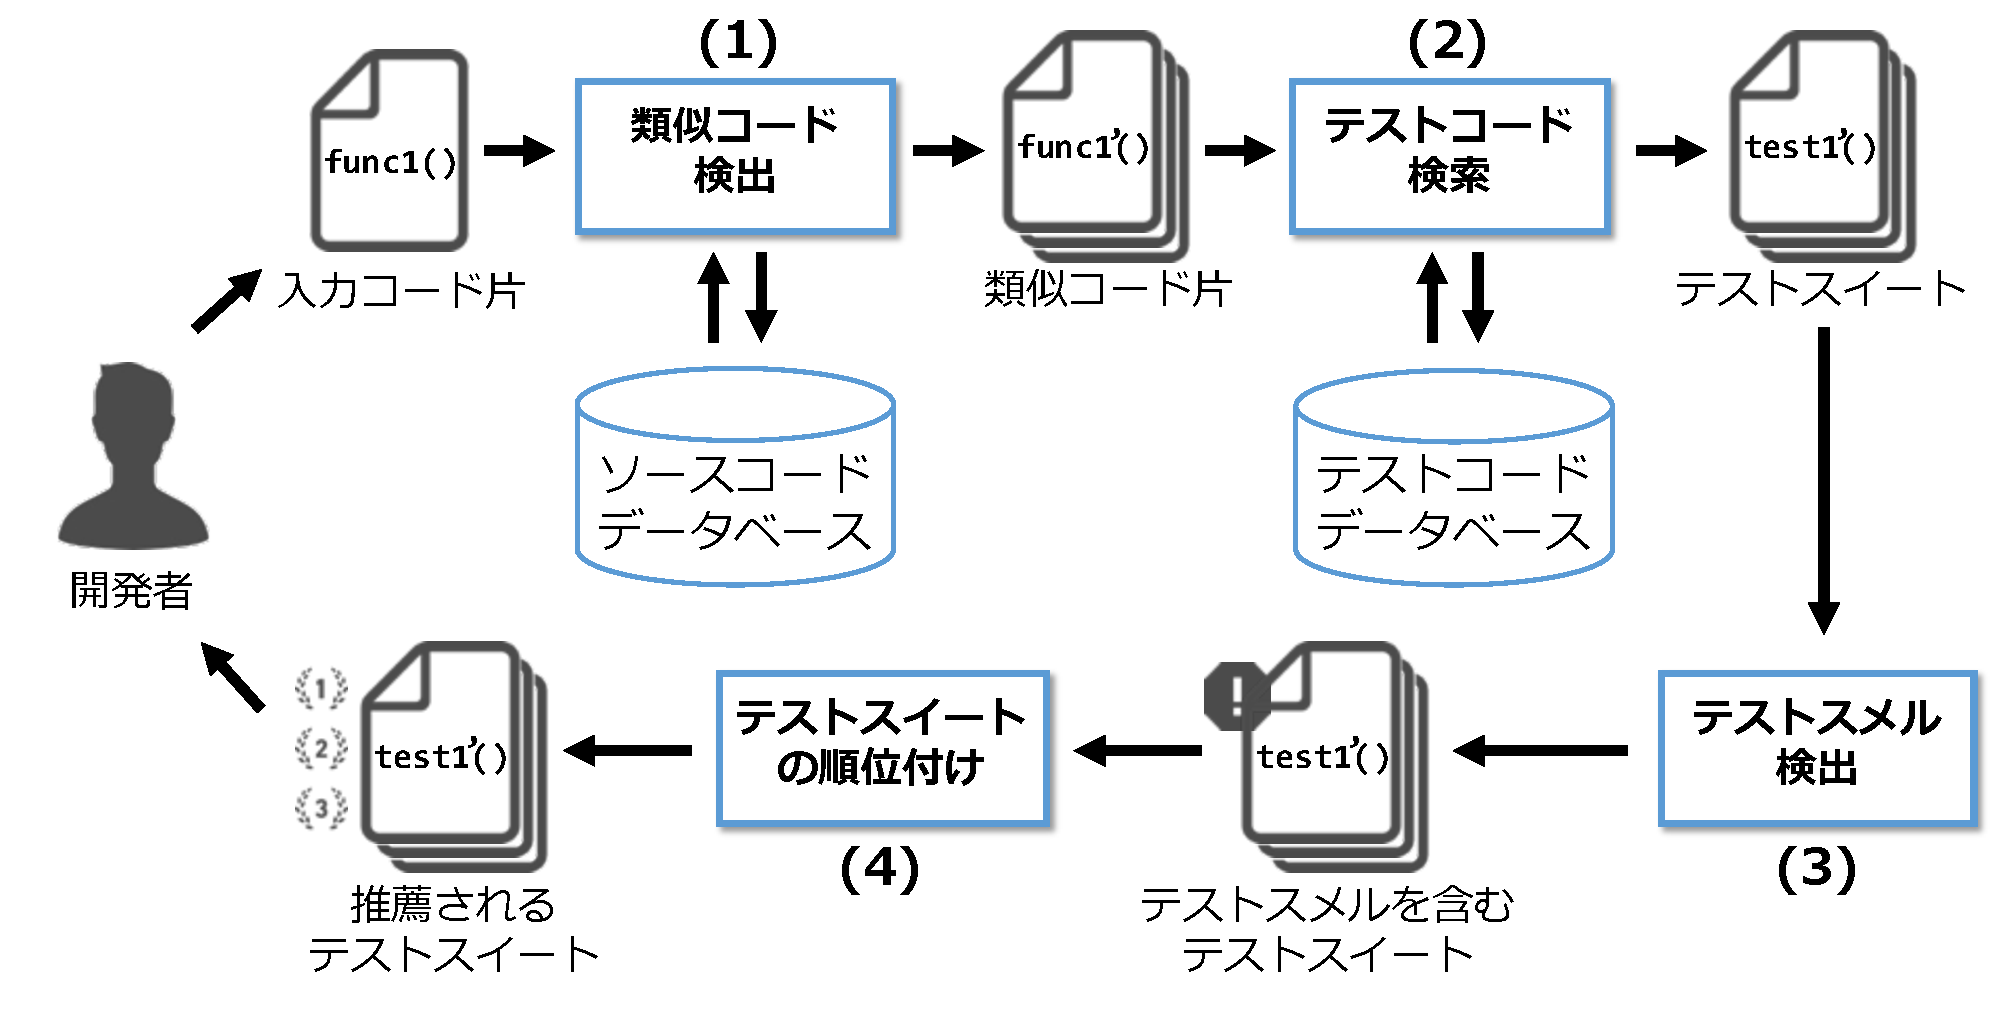
\includegraphics[width=8.5cm]{image/SuiteRec-outline.pdf}}
\caption{{\sf SuiteRec}の概要}
\label{SO}
\end{figure}

\begin{description}
\item[Step1:]類似コード検出ツールを用いて,開発者から与えられた入力コード片に対する類似コード片を検出する.
\item[Step2:]Step1で検出された複数の類似コード片に対するテストスイートをテストコードデータベース内から検索する.
\item[Step3:]Step2で検出された複数のテストスイートをテストスメル検出ツールにかけ,各テストスイートに含まれるテストスメルを検出する.
\item[Step4:]最後に,Step1で得られた類似コード片と入力コード片の類似度とStep3で検出されたテストスメルの数を基に,出力されるテストスイートの順番を並び替える.
\end{description}

以降の節で,各ステップの詳細について説明する.

\subsection{Step1: 類似コード片の検出}

Step1では,開発者から与えられた関数単位のコード片に対して,類似コード片を検出する.本研究では,コードクローン検出ツールとして{\sf NiCad}\cite{b2}を採用した.{\sf NiCad}は,検出対象のコード片のレイアウトを統一的に変換させ,行単位で関数単位のコード片を比較することで,高精度・高再現率でクローンペアの検出するツールである.

{\sf SuiteRec}は,{\sf NiCad}を用いて入力コード片に対する類似コード片を大規模なOSSプロジェクトを保持するソースコードデータベースから検索する.ソースコードデータベースには,テストコードが存在するGithub\footnote{https://github.com/}上の3,205個のOSSプロジェクトのプロダクションコードが格納されている.具体的には,既存のコード検索エンジンで利用されたデータセット\cite{FaCoY}の内,テストフォルダが存在し,JUnitのテスティングフレームワークを採用しているプロジェクトを選択した.

{\sf NiCad}は,一度に検索できるプロジェクトの規模限度がある.そこで,本研究では検索時間を短縮するために,検索対象のプロジェクトに前処理を行い,ソースコードデータベースに格納した.具体的には,大規模なプロジェクトは分割し,小規模なプロジェクトは統合させた状態で検索処理を実行した.さらに,検索処理を複数のプロジェクトに対して並列して走らせることで,現実的な時間での類似コード片の検索を実現した.
\subsection{Step2: テストコードの検索}
\label{step2}

Step2では,Step1で検出された類似コード片に対するテストスイートを検索する.大規模なプロジェクトのテストコードが格納されているテストコードデータベース(以下,TDB)からテストスイートを検出するために,テスト対象コードとテストコードの対応付けを行う.

本研究では,テスト対象コードとテストコードを対応付けるために以下の3つのフェーズを実施する.


\begin{description}
\item[Phase1:]命名規則によるクラス単位で,テストクラスとテスト対象クラスを対応付ける.
\item[Phase2:]テストコードを静的解析し,各テストコードから呼び出されるすべてのテスト対象のメソッド名を収集する.
\item[Phase3:]テストメソッド名を区切り文字や大文字で分割し,テスト対象のメソッド名と部分一致した場合,テストコードとテスト対象コードをメソッド単位で対応付ける.
\end{description}



本研究は,JUnitテスティングフレームワークを用いた単体テストを対象とする.Phase1では,JUnitの命名規則に従ってテストクラス名の先頭または,末尾に``Test''という文字列が含まれるテストクラスを収集し,収集したテストクラスから``Test''を除いたクラス名をテスト対象クラスとする.例えば,テスト対象クラスである``Calculatorクラス''とテストクラスである``CalculatorTestクラス''が対応付けられる.

Phase2では,テストコードをANTLR\footnote{https://www.antlr.org/}を用いて静的解析し,テストメソッド内で呼び出されるテスト対象のメソッド名を取得する.単体テストは,一般的に,図\ref{mapping}の例のようにテストコード内でテスト対象のオブジェクトの生成を行い,テスト対象のメソッド呼び出して実行される.したがって,TCD内のテストコードを静的解析し,テスト対象のメソッド呼び出しを取得することで,テスト対象コードとテストコードを対応付ける.ただし,テストメソッド内では,複数のテスト対象のメソッドが呼び出されていることも考えられるので,Phase3では,さらにテスト対象のメソッド名とテストメソッド名の比較も行う.テストメソッド名の記述方法として,テスト対象メソッドの処理の内容を忠実に表すことが推奨されており,テストメソッド名にテスト対象メソッドの名前が記述されていることが多い\cite{b22}.したがって,テストメソッドの名前を区切り文字や大文字で分割し,テスト対象のメソッド名と部分一致した場合,テストコードとテスト対象コードをメソッド単位で対応付けるように実装した.

\begin{figure}[htbp]
\centerline{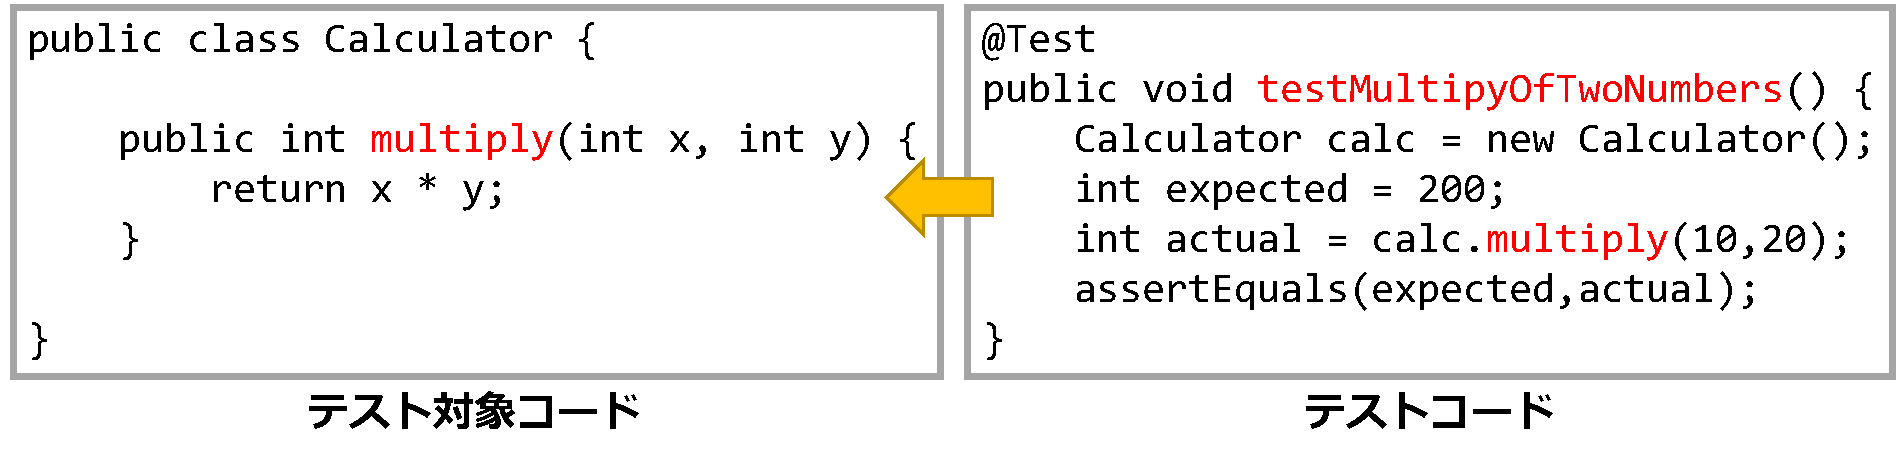
\includegraphics[width=8.5cm]{image/mapping.pdf}}
\caption{テストコードと対象コードの対応付け}
\label{mapping}
\end{figure}

\subsection{Step3: テストスメルの検出}
\label{step3}

Step3では,Step2で検索されたテストスイートに対して,テストスメルを検出する.本研究では,テストスメル検出ツールとして{\sf tsDetect}\footnote{https://testsmells.github.io/}\cite{Peruma}を採用した.{\sf tsDetect}はASTベースの検出手法で実装されたツールであり,19種類のテストスメルを検出できるツールである.また,85\%〜100\%の検出精度と90\%〜100\%の再現率でテストスメルを検出できる.{\sf tsDetect}は,高精度で多くのテストスメルを検出できるので,本研究でも利用した.本研究では,{\sf tsDetect}で検出できる19種類のテストスメルの内,\ref{sec:testsmell}節で説明したテストコードの推薦を考える上で重要な6種類のテストスメルを提示するように実装した.また,再利用対象のテストコードとして相応しくない以下の4つのテストスメルを含むテストコードを事前にTDBから除去し,{\sf SuiteRec}が推薦するテストコードとして出力されないようにした.

\begin{itemize}
\item \textbf{Empty Test} : テストメソッド内にテストの記述が無く,コメントのみが含まれているテストコード
\item \textbf{Ignored Test} : @Ignoreアノテーションがあり,実行されないテストコード
\item \textbf{Redundant Assertion} : 必ずテストが成功する意味のないテストコード
\item \textbf{Unknow Test} : assert文が存在しないテストコード
\end{itemize}

\subsection{Step4: 推薦されるテストスイートの順位付け}
\label{step4}

最後のStep4では,開発者が参考にしたいテストスイートを上位に提示できるようにテストスイートの並び替えを行う.

{\sf SuiteRec}の順位付けは,Step1の入力コード片と類似コード片の類似度とStep3で検出されたテストスメルの数を基に計算する.我々は,以前の調査\cite{fose2019}で,クローンペア間とテストコードの類似度の関係を調査した.具体的には,OSS上に存在する3つの有名Javaプロジェクト内にある両方のコード片にテストコードが存在するコードクローンを対象に,クローンペア間の類似度とそれぞれのコード片に対するテストコードの類似度の関係を調査した.その結果,テストコード間の類似度と対象のクローンペア間の類似度には相関関係があり,クローンペア間の類似度が高いほどテストコードを再利用できる可能性が高いことが分かった.{\sf SuiteRec}では,この結果を基に類似度が高いクローンペアの順にテストスイートを並び替え,さらに類似度が同じ場合,テストスメルの数で推薦するテストスイート順位を決定するように推薦ランキングを実装した.


\section{評価実験}
\label{evaluation}


この章では,{\sf SuiteRec}の有用性を定量的および定性的に評価するために行った評価実験について説明する.

評価実験では,情報科学を専攻するの修士過程の学生10人に対して実験を実施し,{\sf SuiteRec}がテストコードの作成をどの程度支援できるかを評価した.具体的には,被験者に3つのプロダクションコードのテストコードを作成してもらい,{\sf SuiteRec}を使用して作成した場合とそうでない場合で,作成したテストコードを比較することで評価を行う.実験を通してコードカバレッジ,実験タスクを終了するまでの時間および,テストコードの品質に関するデータを収集することで,以下の4つのリサーチクエスチョンに答えることを目指す.

\begin{itemize}
\item \textbf{RQ1: {\sf SuiteRec}は高いカバレッジを持つテストコードの作成を支援できるか?}
\item \textbf{RQ2: {\sf SuiteRec}はテストコードの作成時間を削減できるか?}
\item \textbf{RQ3: {\sf SuiteRec}はテストスメルの数が少ないテストコードの作成を支援できるか?}
\item \textbf{RQ4: {\sf SuiteRec}の利用は,開発者のテストコード作成タスクの認識にどう影響するか?}
\end{itemize}

%以降,\ref{secdataset}節では,評価実験で用いた実験用データセットについて説明する.\ref{sec:process}節では,評価実験1の手順について説明する.最後に4.1.3節で,評価実験1の結果について説明する.


\subsection{評価実験のデータセット}
\label{sec:dataset}

評価実験1では,被験者に3つの実験タスクを割り当てた.以降,これら実験タスクをそれぞれ,タスク1,タスク2,タスク3と呼ぶ.被験者がテストコードを作成するためには,プロダクションコードの仕様を十分に理解しておく必要がある.そこで,本研究ではプロダクションコードとして競技プログラミングをよく用いられる典型的な計算問題を実験タスクとして選択した.また,各タスクの仕様を確認できるように自然言語で記述された仕様書を用意した.3つの各タスクで違いを出すためにタスク1,2,3の順に条件分岐の数を8,16,24と多くなるように設定した.図\ref{task}は,各タスクの概要を示す.

\begin{figure}[htbp]
\centerline{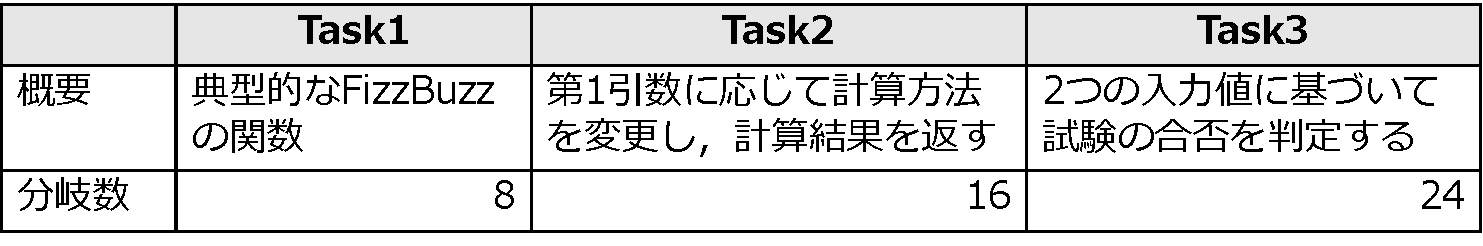
\includegraphics[width=8.5cm]{image/task.pdf}}
\caption{実験タスクの概要}
\label{task}
\end{figure}




\subsubsection{評価実験の手順}
\label{sec:process}

\ref{sec:E1data}節で説明した実験タスクを用いた評価実験1の手順について説明する.まず,被験者間の事前知識の違いによる結果の相違を無くすために,実験前にソフトウェアテストに関する基本的な知識からJUnitの使用に関する30分の講義を実施した.また,被験者に{\sf SuiteRec}の使い方を説明し,実際に練習問題で使用してもらい{\sf SuiteRec}の利用方法とテストコードの作成について十分に理解していることを確認した.

その後,用意した3つの実験タスクに対してテストコードを作成してもらった.被験者には,与えられた3つタスクを{\sf SuiteRec}を使用した場合とそうでない場合でテストコードを作成してもらった.本実験では,タスクの終了は被験者に判断してもらう.具体的には,被験者自身が作成したテストコードのカバレッジ・品質に満足したとき,実験タスクを終了を宣言してもらい,実験タスク開始から終了宣言までの時間をタスク完了までの時間とした.実験時間は1つのタスクにつき最大25分の時間を設け,それ以降はタスクの途中だとしても作業終了してもらった.

我々は,{\sf SuiteRec}の利用効果がタスクによって偏らないように,図\ref{assign}のように被験者を2つのグループに分け,グループによって{\sf SuiteRec}の利用の有無をタスクによって変えるように割り当てた.また,{\sf SuiteRec}を利用した場合の学習効果を防ぐために,3つのタスクで連続して{\sf SuiteRec}を利用しないようにタスクの割り当てを行った.さらに実験中,被験者は過去の回答を参考できないようにした.

\begin{table}[h]
\caption{タスクの割り当て}
\label{assign}
\begin{center}
\begin{tabular}{|c|l|l|l|c|}
\hline
グループ & \multicolumn{2}{c|}{A} & \multicolumn{2}{c|}{B} \\ \hline
& \multicolumn{1}{c|}{タスク} & \multicolumn{1}{c|}{ツール} & \multicolumn{1}{c|}{タスク} & ツール \\ \hline
1回目 & タスク1 & & タスク1 & 〇 \\ \hline
2回目 & タスク2 & \multicolumn{1}{c|}{〇} & タスク2 & \multicolumn{1}{l|}{} \\ \hline
3回目 & タスク3 & & タスク3 & 〇 \\ \hline
\end{tabular}
\end{center}
\end{table}


最後に,実験タスク終了後に被験者にテストコード作成に関するアンケートに答えてもらった.以下に,実施したアンケートの項目を示す.被験者は,これらのアンケート項目に対して5段階評価(強く反対・反対・どちらでもない・賛成・強く賛成)で回答してもらった.




\subsubsection{評価実験1の結果}
\label{sec:process}
本節では,評価実験1の被験者による{\sf SuiteRec}の定量的および定性的評価の結果を,本章の前半で説明した4つのリサーチクエスチョンを用いて説明する.

\paragraph{RQ1: {\sf SuiteRec}は高いカバレッジを持つテストコードの作成を支援できるか?}このRQに答えるために,{\sf SuiteRec}を使用した場合とそうでない場合で,被験者が作成したテストコードのカバレッジを比較した.本実験では,被験者によって提出されたテストコードの命令網羅と分岐網羅の2種類のカバレッジを計算した.カバレッジの計算には,統合開発環境Eclipse\footnote{https://www.eclipse.org/}のプラグインであるEclEmma\footnote{https://www.eclemma.org/}を利用した.図\ref{C0}と図\ref{C1}は,それぞれ被験者による命令網羅と分岐網羅の平均カバレッジを示す.この図から分かるように,命令網羅の割合は3つのタスクすべてにおいてツールを利用した場合とそうでない場合で網羅率にほとんど違いはなく,どのタスクも網羅率が90\%を超えている.図\ref{C1}の分岐網羅についても分岐数が少ないタスク1とタスク2については,ツールを使用した場合とそうでない場合でほとんど差がないことが分かる.しかし,プロダクションコードの分岐数が最も多いタスク3については,実験者の平均カバレッジに10\%以上の差があることが分かった.この結果は,分岐が多いプロダクションコードのテストコードを作成する際に,{\sf SuiteRec}で推薦されるテストコードは,網羅率を向上するのに役に立つことが考えられる.実際に実験後のアンケートの記述欄には,推薦コードによって見落としていたテスト項目をフォローすることができたという報告が複数存在した.


\begin{figure}[htbp]
\centerline{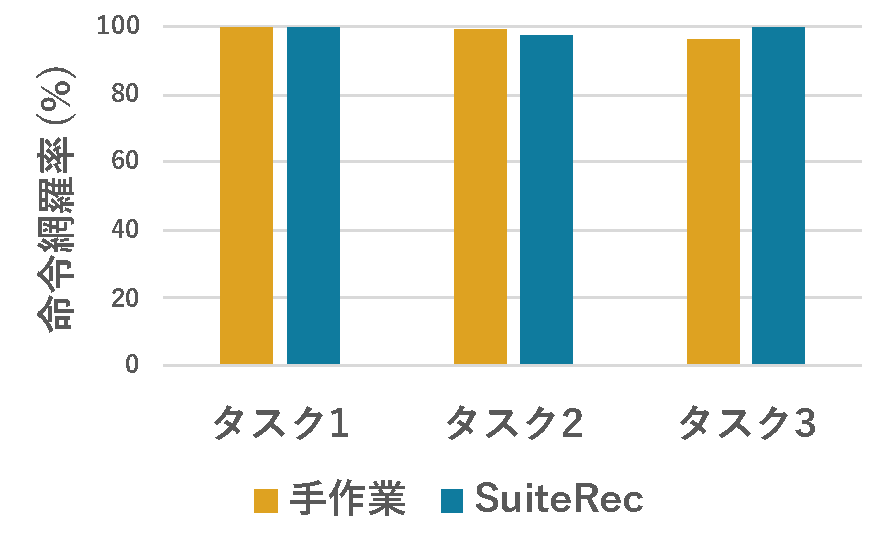
\includegraphics[width=8.5cm]{image/M.pdf}}
\caption{命令網羅の平均カバレッジ}
\label{C0}
\end{figure}

\begin{figure}[htbp]
\centerline{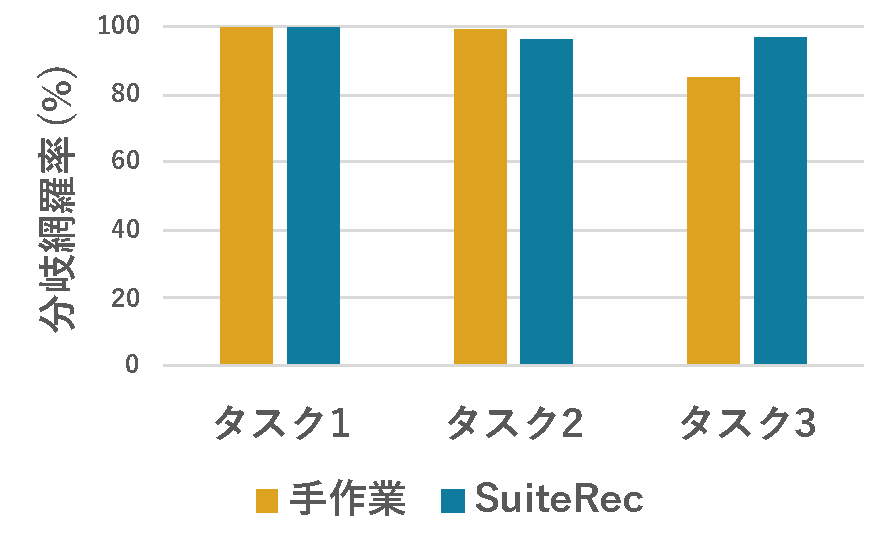
\includegraphics[width=8.5cm]{image/B.pdf}}
\caption{分岐網羅の平均カバレッジ}
\label{C1}
\end{figure}



\begin{breakbox}
\textit{条件分岐が多く複雑なプログラムのテストコードを作成する際,{\sf SuiteRec}の利用はカバレッジ(C1)を向上するのに役立つ可能性がある.}
\end{breakbox}

\paragraph{RQ2: {\sf SuiteRec}はテストコードの作成時間を削減できるか?}このRQを答えるために,{\sf SuiteRec}を使用した場合とそうでない場合で,被験者のテストコード作成タスクが完了するまでに費やした時間を比較した.図\ref{time}は,各被験者のタスク完了までに費やした時間の分布を示す.この図から分かるように,3つのタスクの内2つのタスクで{\sf SuiteRec}を使用した場合は,そうでない場合と比べてテスト作成時間が長いことが分かる.{\sf SuiteRec}を用いた場合,テスト作成に時間がかかる原因として,推薦される複数のテストスイートのソースコードを読んで理解するのに時間がかかったことが考えられる.被験者は多くの場合,推薦されるテストコードをそのままの形で再利用できない.入力したコード片と検出された類似コード片の差分を確認し,テストコードを書き換える必要がある.一方で,タスク2については,{\sf SuiteRec}を利用した場合の方がテスト作成時間が短いことが分かる.我々は,提出されたテストコードを調査したところ,カバレッジに差はないものの{\sf SuiteRec}を使用しない場合は,テストケースの重複が多くなっていることが分かった.この結果は,被験者は無駄なテストケースを多く記述するのに時間を費やした可能性がある.


\begin{figure}[htbp]
\centerline{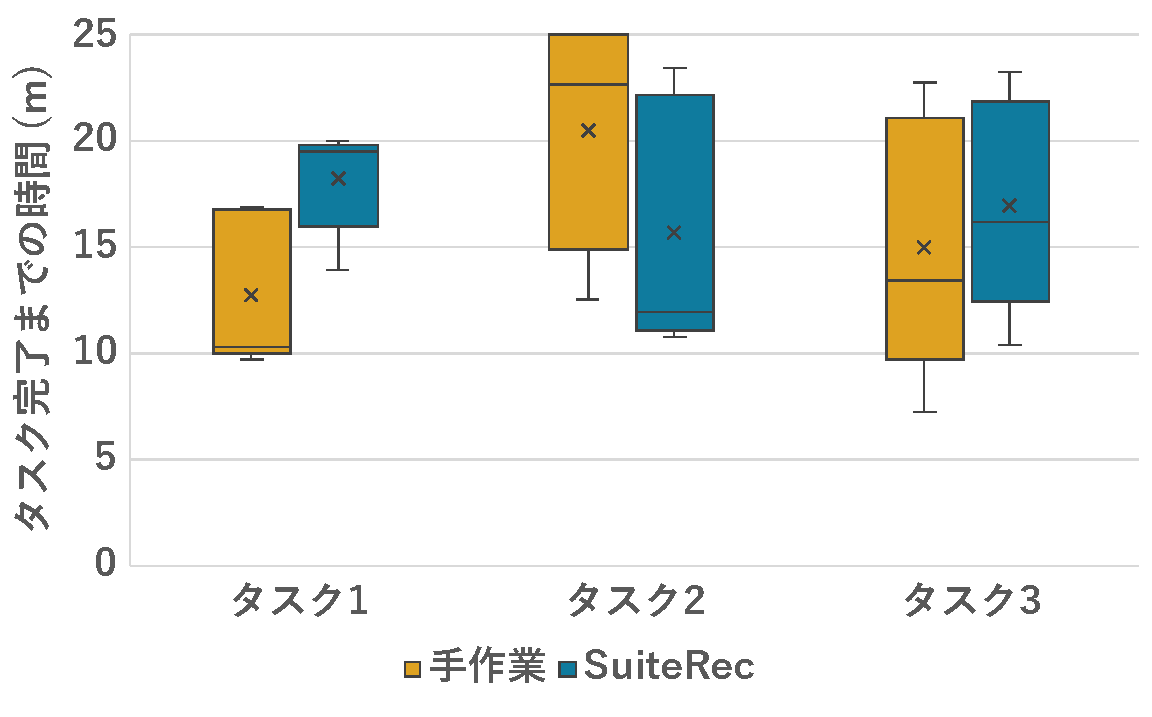
\includegraphics[width=8.5cm]{image/time.pdf}}
\caption{テストコード作成タスク終了までの時間}
\label{time}
\end{figure}


\begin{breakbox}
\textit{{\sf SuiteRec}の利用は,推薦されたテストスイートを理解し変更する必要があるので,開発者はテストコード作成に多くの時間を費やす可能性がある.}
\end{breakbox}



\paragraph{RQ3: {\sf SuiteRec}は,テストスメルの数が少ないテストコードの作成を支援できるか?}このRQに答えるために,{\sf SuiteRec}を使用した場合とそうでない場合で被験者が作成したテストコード内に含まれるテストスメルの数を比較した.図\ref{smell}は,各タスクごとの被験者が提出したテストコード内に含まれていたテストスメルの数の合計を示す.この図から分かるように,すべてのタスクに対して,{\sf SuiteRec}を使用して作成されたテストスイートは,使用しない場合と比べて検出されたテストスメルの数が少ないことが分かる.これは,{\sf SuiteRec}によって推薦されるテストスイートの品質が高く,被験者はそれを再利用することで品質を維持したままテストコードを作成できたと考えられる.また,{\sf SuiteRec}の出力画面で推薦されるテストスイート内に含まれているテストスメルの情報を提示することで,その情報に基づいてテストコードを書き替えることができ,品質が高いテストコードを提出した可能性が考えられる.一方で,{\sf SuiteRec}を使用せずに作成されたテストスイートは,{\sf SuiteRec}を使用して作成されたテストスイートと比べ全体として5倍以上のテストスメルが含まれていた.多く埋め込まれていたテストスメルとして,``Assertion Roulette'', ``Default Test'',``Eager Test''が挙げられる.これは多くの被験者が,初期状態のテストメソッドの名前を変更せず,1つのテストメソッド内でコピーアンドペーストによってassert文を記述していたことが原因だと考えられる.実際に,既存研究でもこれらのテストスメルが,既存プロジェクトで多く検出されていることが報告されている\cite{Peruma}.


\begin{figure}[htbp]
\centerline{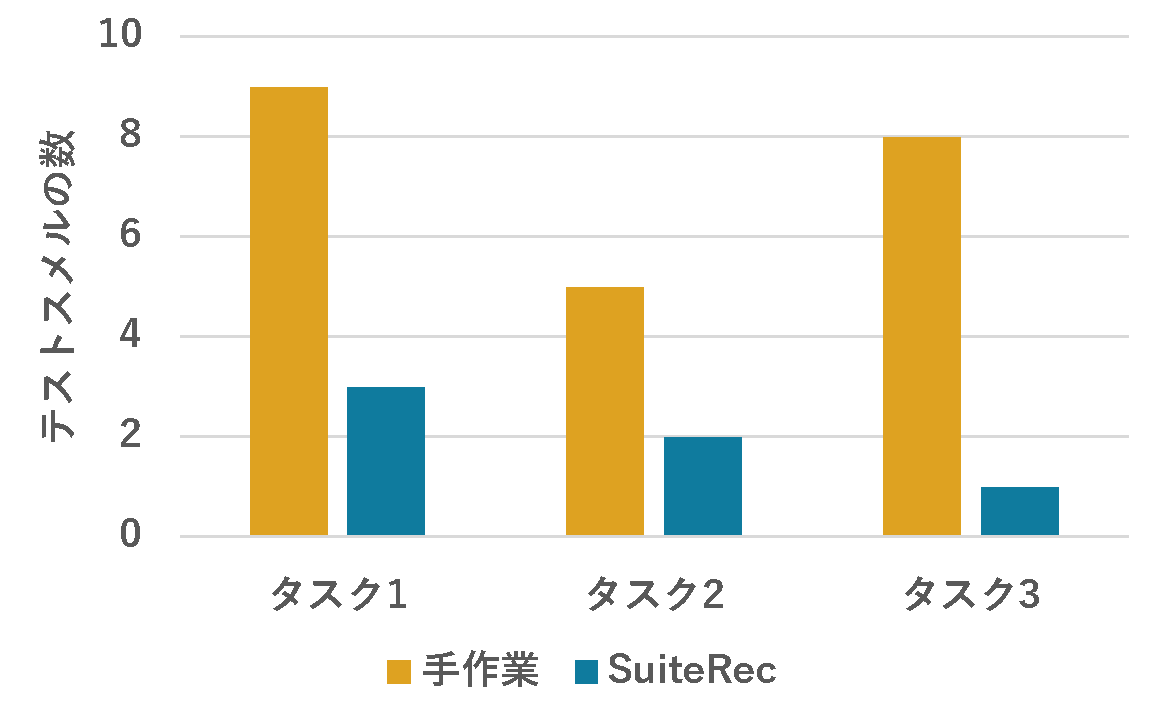
\includegraphics[width=8.5cm]{image/smells.pdf}}
\caption{テストコード内に含まれていたテストスメルの数}
\label{smell}
\end{figure}



\vspace{\baselineskip}

\begin{breakbox}
\textit{開発者は,{\sf SuiteRec}によって推薦される高品質のテストスイートを参考にすることで品質の高いテストコードを作成できる可能性がある.}
\end{breakbox}

\paragraph{RQ4: {\sf SuiteRec}の利用は,開発者のテストコード作成タスクの認識にどう影響するか?}

このRQに答えるために,評価実験の後,被験者に対して実験タスクに関するアンケートを実施した.図\ref{QA}は実施したアンケートの内容とその結果を示す.Q1,Q2の回答から,被験者は,実験タスクを明確に理解し(質問1),実験タスクを終えるのに十分な時間があったことが分かる(質問2).Q1,Q2以外の質問については,{\sf SuiteRec}を使用した場合とそうでない場合で,実験タスクに対する意見に違いがある.

質問3の回答から被験者は,テストコードを作成する際に,{\sf SuiteRec}を用いることでテストコード作成を容易に感じることが分かった.しかし,この結果は実際のタスクの完了までの時間(図\ref{time})とは対照的であり,{\sf SuiteRec}を使用した場合の方がタスクの完了までにかかる時間が長いことが分かる.{\sf SuiteRec}を使用した場合,被験者はテストコードの作成に多くの時間を費やす.しかし,{\sf SuiteRec}を用いたテストコードの作成作業は,単純で繰り返すことが多いので被験者は容易に感じた可能性がある.また,{\sf SuiteRec}によって推薦されたテストスイートがテスト項目を考える上で参考になり,テストスイートの記述には時間がかかるが,全体としては容易な作業だと感じた可能性が高い.

質問4の回答から被験者は,{\sf SuiteRec}を使用した場合,自身で作成したテストコードのカバレッジに自信があることが分かる.一方で,{\sf SuiteRec}を使用しなかった場合,40\%の被験者がネガティブな回答を報告した.しかし,実際に提出されたテストコードのカバレッジには,ほとんど差がないことが分かる(図\ref{C0},\ref{C1}).開発者が自分自身で作成したテストコードのカバレッジに自信を持つことは重要である.開発者は,自分の作成したコードに責任を持ち,不安なくソフトウェアをユーザに提供できることは,ソフトウェアテストを行う目的の1つである.

質問5の回答から,{\sf SuiteRec}を使用せずにテストコードを作成した場合,40\%の被験者が自身の作成したテストコードの品質に自信が持てないことが分かった.実際に,提出されたテストコード内のテストスメルの数も{\sf SuiteRec}を使用した場合よりも多く存在している(図\ref{smell}).開発者は無意識の内にテストスメルを埋め込み,そのテストスメルが後の保守活動を困難にする.{\sf SuiteRec}の利用は,開発者にテストコードの品質に対する意識を与えることでテストメルの数を減らし,作成したコードに対して自信をもたらす.一方で,{\sf SuiteRec}を利用した場合でも品質に関してネガティブな意見も存在した.アンケートの記述項目では,テストスメルの存在は意識できたが具体的にどう修正して無くすことができるのか分からなかったと報告されていた.これは{\sf SuiteRec}の更なる改善の必要性を示しており,各テストスメルに対するリファクタリング方法も提示する機能を追加すべきである.

\begin{figure}[htbp]
\begin{center}
\includegraphics[width=15cm]{image/suiterec-expt.pdf}
\caption{実験後のアンケートの回答}
\label{QA}
\end{center}
\end{figure}

\begin{breakbox}
\textit{{\sf SuiteRec}を利用した場合,開発者はテスト作成タスクを容易だと認識し,作成したテストコードに自信が持てる.}
\end{breakbox}



\section{議論}
\label{discussion}

\section{まとめと今後の課題}
\label{conclusion}


\begin{comment}

以下のテンプレートに従って記述してください.
原稿執筆に際しては,本クラスファイルとともに配布される
テンプレート(\texttt{template.tex})を利用できます.

\begin{verbatim}
\documentclass[technicalreport]{ieicej}
\jtitle{和文題目}
\jsubtitle{和文副題}
\etitle{英文題目}
\esubtitle{英文副題}
\authorlist{%
 \authorentry[densi@firstuniv.ac.jp]
  {電子 花子}{Hanako DENSHI}{Tokyo}
 \authorentry[joho@ohsakacorp.co.jp]
  {情報 太郎}{Jiro JOHO}{Osaka}
}
\affiliate[Tokyo]{第一大学工学部\hskip1zw
  〒105--0123 東京都港区山田1--2--3}
 {Faculty of Engineering, 
  First University\hskip1em
  1--2--3 Yamada, Minato-ku, Tokyo,
  105--0123 Japan}
\affiliate[Osaka]{大阪株式会社開発部\hskip1zw
  〒565--0456 大阪府吹田市河田4--5--6}
 {R\&D Division, Osaka Corporation\hskip1em
  4--5--6 Kawada, Suita-shi,
  565--0456 Japan}
\begin{document}
\begin{jabstract}
和文あらまし
\end{jabstract}
\begin{jkeyword}
和文キーワード
\end{jkeyword}
\begin{eabstract}
英文アブストラクト
\end{eabstract}
\begin{ekeyword}
英文キーワード
\end{ekeyword}
\maketitle
 ---- (略) ----
\end{verbatim}

\begin{itemize}
\item
「技術研究報告」の体裁にするには,
ドキュメントクラスのオプションとして
\texttt{technicalreport} を指定します.

\item
\verb/\jtitle/ には和文題目を指定します.
任意の場所で改行したいときは,\verb/\\/ で改行できます.

\item
\verb/\etitle/ は,英文題目を指定します.

\item
和文副題および英文副題を指定することができます.
それぞれ,\verb/\jsubtitle/ と \verb/\esubtitle/ に
記述します.

\item
和文発表者名および英文発表者名は,以下のように記述します.
発表者名,所属,メールアドレスなどの出力体裁を自動的に整えます.
\begin{verbatim}
\authorlist{%
 \authorentry[メールアドレス]{和文発表者名}
  {英文発表者名}{所属ラベル}
}
\end{verbatim}

\begin{itemize}
\item
第1引き数は,メールアドレスを指定します.
これは省略可能です.

``\texttt{\_}'' を含むメールアドレスの場合は
\begin{verbatim}
 \noexpand\noexpand\noexpand\_
\end{verbatim}
と記述してください.

発表者が複数の場合で,メールアドレスをお持ちでない方がある場合は,
かならず \texttt{[]} を記述した上で,中を空にしてください.
メールアドレスは1人につき1つだけ記述します.
1人につき複数のアドレスには対応していません.

メールアドレスの記述が原因でエラーを生じたり,
{\bfseries 出力が望み通りの結果にならない場合}は,
\verb/\MailAddress/ に直接記述してください.
\begin{verbatim}
 \MailAddress{$\dagger$name@xx.yy.zz.jp}
\end{verbatim}

\item
第2引き数は和文発表者名を指定します.
{\bfseries 姓と名の間に必ず半角のスペースを挿入}してください
(スペースを挿入し忘れた場合には,ワーニングが出力されます).

\item
第3引き数は英文発表者名を指定します.
ファミリーネームは大文字で記述します.

\item
第4引き数は発表者の所属ラベルを指定します.
このラベルは,後述する \verb/\affiliate/ の第1引き数に対応します.
ラベルは大学名,企業名,地名などを表す簡潔なものにしてください.
複数の所属がある場合には,カンマ ``,'' でラベルを区切って記述します.

{\bfseries 発表者が一人で所属がない場合}は,
\texttt{none} と指定します.

{\bfseries 発表者が複数で所属のない方がいる場合}は,
\texttt{none} 以外の適当なラベルを付けたうえで,
\verb/\affiliate/ は記述しません.

ラベルの前後やカンマの後ろに余分なスペースを入れないでください.
\verb/{Tokyo}/ と \verb*/{Tokyo }/ は所属が違うものと判断します.
\end{itemize}

\item
和文発表者名および英文発表者名を任意の場所で改行する必要が生じた場合は,
それぞれ \verb/\alignorder/,\verb/\breakauthorline/ コマンドで
制御することができます.
\begin{verbatim}
\alignorder=3
\end{verbatim}
と記述すれば,和文発表者名のリストを 1 行に 3 名ずつ並べます.

また,
\begin{verbatim}
\breakauthorline{3}
\end{verbatim}
と記述すれば,英文発表者名の 3 人目の後ろで改行します.
カンマで区切って複数の数字を指定することもできます.

\item
所属は \verb/\affiliate/ に指定します.
\begin{verbatim}
 \affiliate[ラベル]
  {和文勤務先\hskip1zw 和文連絡先住所}
  {英文勤務先\hskip1em 英文連絡先住所}
\end{verbatim}
第1引き数に \verb/\authorentry/ で指定したラベルを記述します.
ラベルの前後に余分なスペースを挿入しないでください.
第2引き数に和文の所属を,第3引き数に英文所属を指定します.
勤務先と連絡先住所を \verb/\hskip1zw/ などを使うことによって
少し間を空けてください.
\verb/\authorentry/ に記述したラベルの出現順に記述してください.

\item
和文の「あらまし」「キーワード」は,\texttt{jabstract} 環境,
\texttt{jkeyword} 環境にそれぞれ記述します.また,
英文の「abstract」「key words」は,\texttt{eabstract} 環境,
\texttt{ekeyword} 環境にそれぞれ記述します.
\end{itemize}

\subsection{論文誌の体裁に変更する場合}

「論文」,「レター」などの論文誌の体裁に変更する場合は,
以下の点に注意してください.
\begin{itemize}
\item
\verb/\jsubtitle/ と \verb/\esubtitle/ は記述しても無効になります.

\item
\verb/\affiliate/ の和文連絡先住所を簡略化する必要があります.
「和文論文誌投稿のしおり」
(http://www.ieice.or.jp\slash{}jpn\slash{}ronbun.html),
またはバックナンバーを参照してください.

\item
\texttt{jabstract} 環境は \texttt{abstract} 環境と見なしますが,
\texttt{eabstract} 環境は,最終ページに一段組で出力されます.

\item
\texttt{jkeyword} 環境は \texttt{keyword} 環境と見なしますが,
\texttt{ekeyword} 環境は,最終ページに一段組で出力されます.
\end{itemize}


\begin{table}[tb]% Table 1
\caption{サイズと行間の変更}
\ecaption{Settings of size and baselineskip.}
\label{table:1}
\begin{center}
\begin{tabular}{ll}
\Hline
\noalign{\vskip.5mm}
\verb/\normalsize/   & 9\,pt(5.125\,mm) \\
\verb/\small/        & 8\,pt(4.5\,mm) \\
\verb/\footnotesize/ & 7\,pt(4\,mm) \\
\verb/\scriptsize/   & 6\,pt(8\,pt)\\
\verb/\tiny/         & 5\,pt(6\,pt) \\
\verb/\large/        & 10\,pt(5.5\,mm) \\
\verb/\Large/        & 11\,pt(6.75\,mm) \\
\verb/\LARGE/        & 12\,pt(8.25\,mm) \\
\verb/\huge/         & 14\,pt(25\,pt) \\
\verb/\Huge/         & 17\,pt(30\,pt) \\
\noalign{\vskip.5mm}
\Hline
\end{tabular}%
\end{center}
\end{table}


\subsection{文字サイズと行間}

本文の活字の大きさを,9\,pt に設定しています.
したがって,\verb/\normalsize/,\verb/\small/ などのサイズおよび行間を
表~\ref{table:1} に示すように変更しています.

\subsection{見出しの字どり}

\verb/\section/,\verb/\subsection/ などについては,
本誌のスタイルにより,その見出しが4字以下の際,5字どりになるように
設定しています({\bfseries \ref{sec:etc}} の見出しを参照).

\subsection{ディスプレー数式}

数式の頭は左端から1字下げのところに,また,数式番号は
右端から1字入ったところに出力される設定になっています.
この設定を前提に数式の折り返しを調整してください.
\verb/\documentclass/ のオプションとして 
\texttt{fleqn} を指定する必要はありません.

技術研究報告原稿は二段組みで一段の左右幅がせまいため,
数式と数式番号が重なったり,数式がはみ出したりすることが
頻繁に生じると思われます.
\texttt{Overfull} \verb/\hbox/ のメッセージには特に気をつけてください.

数式記述の際のヒントについては,{\bfseries \ref{sec:equation1}} および
{\bfseries \ref{sec:equation2}} が参考になるかもしれません.

\subsection{図表とキャプション}

図表を置く位置,キャプションの記述,図の取り込み,
表の記述などについて説明します.

\subsubsection{図表を置く位置}

\texttt{float} 環境は,それが初めて引用される段落の
直後または直前あたりに挿入することが基本ですが,
二段組みの場合は,それが初めて引用されるページより
前に置くことが必要になることがあります.
図表の出力位置は,図表の参照と同じページか,
無理な場合は次のページに置くことが基本ですから,
二段組みの図表の場合は,\texttt{float} 環境を記述する位置の
試行錯誤が必要となることがあります.

図表の出力位置を指定するオプションとして,\texttt{[h]} の使用は避け,
\texttt{[tb]},\texttt{[tbp]} などを指定して,
ページの天か地に置くことを基本にしてください.

\subsubsection{キャプションとラベル}

図表のキャプションは,和文と欧文で指定する必要があるため,
\verb/\ecaption/ というマクロを用意しました.
使い方は \verb/\caption/ と同じです.
図~\ref{fig:1} のように記述してください.


\begin{figure}[t]%fig.1
\setbox0\vbox{%
\hbox{\verb/\begin{figure}[tb]/}
\hbox{\verb/%\capwidth=60mm/}
\hbox{\verb/%\ecapwidth=60mm/}
\hbox{\verb/\vspace{45mm}/}
\hbox{\verb/\caption{図キャプションの例}/}
\hbox{\verb/\label{fig:1}/}
\hbox{\verb/\ecaption{An example of caption./}
\hbox{\verb/\end{figure}/}
}
\begin{center}
\fbox{\box0}
\end{center}
\caption{図キャプションの例}
\label{fig:1}
\ecaption{An example of caption.}
\end{figure}


\begin{itemize}
\item
キャプションの幅は,一段の場合には一段の幅に,
二段ぬきの場合はテキストの幅の3分2に設定しています.

\item
キャプションを任意の場所で改行したい場合は,
\verb/\\/ を使って改行することができます.
標準の \LaTeXe\ でこういう使い方をすると,
エラーになるので注意してください.

\item
また,\verb/\capwidth/ および \verb/\ecapwidth/ に長さを指定すれば,
その幅で折り返すことができます.
\begin{verbatim}
\capwidth=60mm
\end{verbatim}
これは \verb/\caption/ コマンドの前に指定します.

\item
\verb/\label/ を記述する場合は,
必ず \verb/\caption/ の直後に置きます.
上におくと \verb/\ref/ で正しい番号を参照できません.
\end{itemize}

\subsubsection{図の取り込み}

図の取り込みに関しては,「技術研究報告」では,
「発表者が作成した原稿をそのままオフセット印刷します」ので,
図はどのような形式のものでも構いません.
ここではPDF形式の図を読み込む場合の説明を簡単にします.

例えば,パッケージとして
\begin{verbatim}
\usepackage[dvipdfmx]{graphicx}
\end{verbatim}
を指定し,
\begin{verbatim}
\begin{figure}[tb]
\begin{center}
 \includegraphics{file.pdf}
\end{center}
\caption{}
\ecaption{}
\end{figure}
\end{verbatim}
のような使い方をします.

詳しくはTeX Wiki\cite{texwiki}を参照されることを勧めます.
また文献では\cite{FMi1,latex,FMi2,Nakano,otobe,Okumura3,Eguchi}などが
あります.

\subsubsection{表の記述}

表は \verb/\small/(8\,pt)で組まれるように設定しています.

例えば,以下のように記述します.
\begin{verbatim}
\begin{table}[tb]
\caption{和文キャプション}
\label{table:1}
\ecaption{英文キャプション}
\begin{center}
 \begin{tabular}{|c|c|c|}
 \Hline %% ←
  A & B & C \\
 \hline
  x & y & z\\
 \Hline %% ←
 \end{tabular}
\end{center}
\end{table}
\end{verbatim}

\verb/\caption/ は tabular 環境の上に記述します.
本誌では,表の罫の一番上と一番下を太くします.
このため \verb/\Hline/ というマクロを使用してください.
これは
\begin{verbatim}
\def\Hline{\noalign{\hrule height 0.4mm}}
\end{verbatim}
と定義してあります(表~\ref{table:1},\ref{table:2} 参照).
\verb/\hline/ の太さは 0.1\,mm です.

\subsection{文献リストと文献番号の参照}

\BibTeX\ を利用しない場合は,
文献リストの記述\ddash 
著者名とイニシャル,表題・書名,雑誌名・発行所および雑誌名の略語,巻,号,
ページ,発行年などの体裁\ddash 
は「原稿の書き方」に従ってください.

\BibTeX\ を使って,
文献用データベースファイルから文献リストを作成する場合は,
文献用スタイルとして \texttt{tieice.bst} が利用できます.
標準でインストールされているようです.
得られた文献リストを必要に応じて修正してください.
\BibTeX\ の使い方は,文献 \cite{latex,FMi1,Okumura3} などを
参考にしてください.

文献引用のコマンドは,
\texttt{cite.sty} および \texttt{citesort.sty} に手を加えたものを
使用しています.例えば,
\verb/\cite{/\allowbreak
\texttt{latex,}\allowbreak
\texttt{FGo1,}\allowbreak
\texttt{PEn,}\allowbreak
\texttt{Fujita5,}\allowbreak
\texttt{tex}\allowbreak
\verb/}/ と記述すれば,
``\cite{latex}, \cite{FGo1}, \cite{PEn}, 
\cite{Fujita5}, \cite{tex}'' となるところを,
``\cite{latex,FGo1,PEn,Fujita5,tex}'' のように,
番号順に並べ変え,かつ番号が続く場合は ``〜'' でつなぎます.

\subsection{定理,定義などの環境}

定理,定義,命題などの定理型環境を
記述するには \verb/\newtheorem/(文献\cite{latex,FMi1}参照)が
利用できますが,下の出力例のように,本誌のスタイルにあわせて,
\LaTeXe\ の標準と異なり,環境の上下の空きやインデントを変更し,
見出しはゴシックとならず,本文の欧文もイタリックになりません.

例えば,
\begin{verbatim}
\newtheorem{teiri}{定理}
%\thmbracket{(}{)}
\begin{teiri}
これは ``定理'' の例です.
このような出力になります.
text in Roman typeface.
\end{teiri}
\end{verbatim}
とすれば,
\newtheorem{teiri}{定理}%
%\thmbracket{(}{)}
\begin{teiri}
これは ``定理'' の例です.このような出力になります.
text in Roman typeface.
\end{teiri}
と出力されます.

また,\underline{(}ステップ1\underline{)}のように,
前後の括弧を変えたいときは,
\verb/\thmbracket{(}{)}/ のように \verb/\thmbracket/ の2つの引き数に
前後の括弧をそれぞれ記述します.

\subsection{脚注と脚注マーク}
\label{sec:footnote}

脚注マークは ``$^{\mbox{\tiny (注1)}}$'' という形で出力されます.

\subsection{\texttt{verbatim} 環境}

\texttt{verbatim} 環境のレフトマージン,行間,サイズを
変更することができます\cite{Okumura3}.デフォルトは
\begin{verbatim}
\verbatimleftmargin=0pt
 % レフトマージンは 0pt 
\def\verbatimsize{\normalsize}
 % 本文と同じサイズ
\verbatimbaselineskip=\baselineskip
 % 本文と同じ行間
\end{verbatim}
ですが,それぞれパラメータやサイズ指定を変更することができます.
\begin{verbatim}
\verbatimleftmargin=2zw
% --> レフトマージンを2字下げに
\def\verbatimsize{\small}
% --> 文字の大きさを \small に
\verbatimbaselineskip=3mm
% --> 行間を 3mm に
\end{verbatim}

%\subsection{\texttt{otf} パッケージ}
%% --> 印刷用でないのでこの記述はいらないと思われる
%\texttt{otf.sty} を利用される場合は,以下のような
%オプションをつけることを勧めます.
%\begin{verbatim}
%EUC SJIS の場合
%\usepackage[jis2004,scale=0.985678]{otf}
%UTF の場合
%\usepackage[uplatex,jis2004,
%   scale=0.948427]{otf}
%\end{verbatim}

\subsection{その他}
\label{sec:etc}

\subsubsection{\IEICEJcls\ で定義しているマクロ}

\begin{enumerate}
\item
「証明終」を意味する記号 ``$\Box$'' を出力するマクロとして
\verb/\QED/ を定義してあります\cite{tex}.
\verb/\hfill$\Box$/ では,この記号の直前の文字が行末に来る場合,
記号が行頭に来てしまいますので,\verb/\QED/ を使ってください.
``$\Box$'' を出力するには,パッケージとして
\begin{verbatim}
\usepackage{latexsym}
\end{verbatim}
が必要です.

\item
\verb/\onelineskip/,\verb/\halflineskip/ という行間スペースを
定義しています.
その名のとおり,1行空け,半行空けに使ってください.
和文の組版の場合は,こうした単位の空け方が好まれます.

\item
2倍ダッシュの``\ddash ''は,
\verb/\ddash/ というマクロを使ってください(\ref{sec:hyouki} 参照).
---を2つ重ねると,その間に若干のスペースが入ることがあり
見苦しいからです.

\item
このクラスファイルではこのほかにあらかじめ,
\verb/\RN/,\verb/\FRAC/,\verb/\MARU/,\verb/\kintou/,
\verb/\ruby/ というというマクロ\cite{tex,Okumura3}を
定義しています(表~\ref{table:2}).
\end{enumerate}


\begin{table}[t]% Table 2
\caption{その他のマクロ}
\ecaption{Miscellaneous macros.}
\label{table:2}
\begin{center}
\begin{tabular}{c|c}
\Hline
\verb/\RN{2}/ & \RN{2} \\
\verb/\RN{117}/ & \RN{117} \\
\verb/\FRAC{$\pi$}{2}/ & \FRAC{$\pi$}{2}\\
\verb/\FRAC{1}{4}/ & \FRAC{1}{4} \\
\verb/\MARU{1}/ & \MARU{1}\\
\verb/\MARU{a}/ & \MARU{a}\\
\verb/\kintou{4zw}{記号例}/ & \kintou{4zw}{記号例}\\
\verb/\ruby{砒}{ひ}\ruby{素}{そ}/ & \ruby{砒}{ひ}\ruby{素}{そ}\\
\Hline
\end{tabular}%
\end{center}
\end{table}


\subsubsection{\AmSLaTeX\ について}

数式のより高度な記述のために,\AmSLaTeX\ の
パッケージ(文献\cite{FMi1,otobe}参照)を使う場合には,
パッケージとして
\begin{verbatim}
\usepackage[fleqn]{amsmath}
\end{verbatim}
が必要です.この場合,オプションとして
\texttt{[fleqn]} を必ず指定してください.

\texttt{amsmath} パッケージは,多くのファイルを読み込みますが,
ボールドイタリックだけを使いたい場合は,
\begin{verbatim}
\usepackage{amsbsy}
\end{verbatim}
で済みます.

また,記号類だけを使いたい場合は,
\begin{verbatim}
\usepackage{amssymb}
\end{verbatim}
で済みます.

なお,\LaTeXe\ では \verb/\mbox{\boldmath $x$}/ に代えて,
\verb/\boldsymbol{x}/ を使うことを勧めます.
これならば,数式の上付き・下付きで使うと文字が小さくなります.

%% 以下は 3.3 例1〜3 を除いて,ieicej.cls 付属の readme.tex と同じ
\section{タイピングの注意事項}
\label{sec:typesetting}

\subsection{美しい組版のために}
\label{sec:hyouki}

\begin{enumerate}
\item
和文の句読点は,``\makebox[1zw][c]{,}'' ``\makebox[1zw][c]{.}''%
(全角記号)を使用してください.
和文中では,欧文用のピリオドとカンマ,``,'' ``.'' ``('' ``)''(半角)は
使わないでください.

\item
括弧類は,和文中で欧文を括弧でくくる場合は
全角の括弧を使用してください.
欧文中ではすべて半角ものを使用してください.

\noindent
例:スタイル(Style)ファイル / some (Style) files

上の例にように括弧のベースラインが異なります.

\item
ハイフン(\texttt{-}),二分ダッシュ(\texttt{--}),
全角ダッシュ(\texttt{---}),二倍ダッシュ(\verb/\ddash/)の
区別をしてください.

ハイフンはwell-knownなど一般的な欧単語の連結に,
二分ダッシュはpp.298--301のように範囲を示すときに,
全角ダッシュは欧文用連結のem-dash(---)として,
二倍ダッシュは和文用連結として使用してください.

\item
アラインメント以外の場所で,空行を広くとるため,\verb/\\/ による
強制改行を乱用するのはよくありません.

空行の直前に \verb/\\/ を入れたり,
\verb/\\/ を2つ重ねれば,確かに縦方向のスペースが広がりますが,
\texttt{Underfull} \verb/\hbox/ のメッセージがたくさん出力されて,
重要なメッセージを見落としがちになります\cite{jiyuu}.

\item
\verb*/( word )/ のように ``( )'' 内や ``( )'' 内の単語の前後に
スペースを入れないでください.

\item
プログラムリストなど,インデントが重要なものは,
力わざ(\verb/\hspace*{??mm}/ の使用や \verb/\\/ などによる強制改行)で
整形するのではなく,\texttt{list} 環境や \texttt{tabbing} 環境などを
使って赤字が入っても修正がしやすいように記述してください.
\end{enumerate}

\subsection{数式の記述}
\label{sec:equation1}

\begin{enumerate}
\item
数式モードの中でのハイフン,二分ダッシュ,
マイナスの区別をしてください.

例えば,\par
\noindent
\verb/$A^{\mathrm{b}\mbox{\scriptsize -}/\hfil\break
 \verb/\mathrm{c}}$/\par
\noindent
\hspace{2zw}$A^{\mathrm{b}\mbox{\scriptsize -}\mathrm{c}}$
 $\Rightarrow$ ハイフン\par
\noindent
\verb/$A^{\mathrm{b}\mbox{\scriptsize --}/\hfil\break
 \verb/\mathrm{c}}$/\par
\noindent
\hspace{2zw}$A^{\mathrm{b}\mbox{\scriptsize --}\mathrm{c}}$
 $\Rightarrow$ 二分ダッシュ\par
\noindent
\verb/$A^{b-c}$/\par
\noindent
\hspace{2zw}$A^{b-c}$ $\Rightarrow$ マイナス\par
となります.それぞれの違いを確認してください.

\item
数式の中で,\verb/<,>/ を括弧のように使用することがよくみられますが,
数式中ではこの記号は不等号記号として扱われ,その前後にスペースが入ります.
このような形の記号を括弧として使いたいときは,
\verb/\langle/($\langle$),\verb/\rangle/($\rangle$)を
使うようにしてください.

\item
複数行の数式でアラインメントをするときに
数式が $+$ または $-$ で始まる場合,$+$ や $-$ は単項演算子と
みなされます(つまり,「$+x$」と「$x+y$」の $+$ の前後のスペースは
変わります).したがって,複数行の数式で $+$ や $-$ が先頭にくる場合は,
それらが2項演算子であることを示す必要があります\cite{latex}.
\begin{verbatim}
\begin{eqnarray}
y &=& a + b + c + ... + e\\
  & & \mbox{} + f + ... 
\end{eqnarray}
\end{verbatim}

\item
\TeX\ は,段落中の数式の中(\verb/$...$/)では改行を
うまくやってくれないことがあるので,その場合には \verb/\allowbreak/ を
使用することを勧めます\cite{Abrahams}.
\end{enumerate}

\subsection{長い数式の処理}
\label{sec:equation2}

数式と数式番号が重なったり数式がはみ出したりする場合の
対処策を,いくつか挙げます.

\halflineskip

\noindent
{\bfseries 例1}\hskip1zw \verb/\!/ で縮める.
\begin{equation}
 y=a+b+c+d+e+f+g+h+i+j+k+l+m
% \hskip-10mm %% --> oppress `Overful \hbox ...' message 
\end{equation}
のように数式と数式番号が重なるか,かなり接近する場合は,
まず,2項演算記号や関係記号の前後を,
\verb/\!/ ではさんで縮める方法があります.
\begin{verbatim}
\begin{equation}
 y\!=\!a\!+\!b\!+\!c\!+\! ... \!+\!m
\end{equation}
\end{verbatim}
\begin{equation}
 y\!=\!a\!+\!b\!+\!c\!+\!d\!+\!e\!+\!f\!+\!g\!+\!h
     \!+\!i\!+\!j\!+\!k\!+\!l\!+\!m
\end{equation}

\halflineskip

\noindent
{\bfseries 例2}\hskip1zw \texttt{eqnarray} 環境を使う.

上のようにして縮めても,なお重なったりはみ出してしまう場合は,
\texttt{eqnarray} 環境を使って
\begin{verbatim}
\begin{eqnarray}
 y &=& a+b+c+d+e+f+g+h\nonumber\\
   & & \mbox{}+i+j+k+l+m
\end{eqnarray}
\end{verbatim}
と記述すれば,
\begin{eqnarray}
 y &=& a+b+c+d+e+f+g+h\nonumber\\
   & & \mbox{}+i+j+k+l+m
\end{eqnarray}
となります.

\halflineskip

\noindent
{\bfseries 例3}\hskip1zw \verb/\mathindent/ を変更する.

数式を途中で切りたくない場合は
\begin{verbatim}
\mathindent=0zw % <-- <1>
\begin{equation}
 y=a+b+c+d+e+f+g+h+i+j+k+l+m
\end{equation}
\mathindent=1zw % <-- <2> デフォルト
\end{verbatim}
と記述すれば(\texttt{<1>}),
\mathindent=0zw
\begin{equation}
 y=a+b+c+d+e+f+g+h+i+j+k+l+m
\end{equation}
\mathindent=1zw
となって,数式の頭が左端にきます.
この場合,その数式のあとで \verb/\mathindent/ を
元に戻すことを忘れないでください(\texttt{<2>}).

\halflineskip

\noindent
{\bfseries 例4}\hskip1zw \verb/\lefteqn/ を使う.
\begin{equation}
 \int\!\!\!\int_S \left(\frac{\partial V}{\partial x}
 - \frac{\partial U}{\partial y}\right)dxdy
  = \oint_C \left(U \frac{dx}{ds}
    + V \frac{dy}{ds}\right)ds
 \hskip-10mm %% --> oppress `Overful \hbox ...' message 
\end{equation}

上のように,$=$ までが長くて,数式がはみ出したり,
数式と数式番号がくっつく場合には,\verb/\lefteqn/ を使って
\begin{verbatim}
\begin{eqnarray}
 \lefteqn{
  \int\!\!\!\int_S 
  \left(\frac{\partial V}{\partial x}
  -\frac{\partial U}{\partial y}\right)
  dxdy
 }\quad\nonumber\\
 &=& \oint_C \left(U \frac{dx}{ds}
      + V \frac{dy}{ds}\right)ds
\end{eqnarray}
\end{verbatim}
と記述すれば,
\begin{eqnarray}
 \lefteqn{
  \int\!\!\!\int_S 
  \left(\frac{\partial V}{\partial x}
  -\frac{\partial U}{\partial y}\right)
  dxdy
 }\quad\nonumber\\
 &=& \oint_C \left(U \frac{dx}{ds}
      + V \frac{dy}{ds}\right)ds
\end{eqnarray}
のような形にできます.

\halflineskip

\noindent
{\bfseries 例5}\hskip1zw \verb/\arraycolsep/ を変える.
\begin{equation}
A = \left(
  \begin{array}{cccc}
   a_{11} & a_{12} & \ldots & a_{1n} \\
   a_{21} & a_{22} & \ldots & a_{2n} \\
   \vdots & \vdots & \ddots & \vdots \\
   a_{m1} & a_{m2} & \ldots & a_{mn} \\
  \end{array}
    \right)
 \label{eq:ex1}
\end{equation}

上の行列は \texttt{array} 環境を使って記述しましたが,
\texttt{array} 環境を使っていて数式がはみ出す場合は,
数式全体のフォントサイズを変える前に,
\begin{verbatim}
\begin{equation}
\arraycolsep=3pt %                 <-- <1>
A = \left(
  \begin{array}
   {@{\hskip2pt}cccc@{\hskip2pt}}% <-- <2> 
   a_{11} & a_{12} & \ldots & a_{1n} \\
   a_{21} & a_{22} & \ldots & a_{2n} \\
   \vdots & \vdots & \ddots & \vdots \\
   a_{m1} & a_{m2} & \ldots & a_{mn} \\
  \end{array}
    \right) 
\end{equation}
\end{verbatim}
\texttt{<1>} のように,\verb/\arraycolsep/ の値(デフォルトは5\,pt)を
小さくしてみるか,
\texttt{<2>} のように \texttt{@} 表現を使うことができます.
\begin{equation}
\arraycolsep=3pt
A = \left(
  \begin{array}{@{\hskip2pt}cccc@{\hskip2pt}}
   a_{11} & a_{12} & \ldots & a_{1n} \\
   a_{21} & a_{22} & \ldots & a_{2n} \\
   \vdots & \vdots & \ddots & \vdots \\
   a_{m1} & a_{m2} & \ldots & a_{mn} \\
  \end{array}
    \right)
 \label{eq:ex2}
\end{equation}
式 (\ref{eq:ex1}) と式 (\ref{eq:ex2}) を比べてください.

\makeatletter\ifx\@mathmargin\undefined\makeatother

\halflineskip

\noindent
{\bfseries 例6}\hskip1zw \verb/\quad/ の定義を変える.

行列を記述する場合に使用する \verb/\matrix/,
\verb/\pmatrix/ はコラムの間に \verb/\quad/ が挿入されているので,
間隔を縮めるには,ディスプレー数式環境の中で,
\verb/\def\quad/ の定義を変えてみて下さい.例えば
\begin{equation}
 A = \pmatrix{
      a_{11} & a_{12} & \ldots & a_{1n} \cr
      a_{21} & a_{22} & \ldots & a_{2n} \cr
      \vdots & \vdots & \ddots & \vdots \cr
      a_{m1} & a_{m2} & \ldots & a_{mn} \cr
     }
\end{equation}
のような \verb/\pmatrix/ で記述した行列式で,
\verb/\quad/ の定義を変更すると
\begin{verbatim}
\begin{equation}
 \def\quad{\hskip.5em\relax}
 %% デフォルトは \hskip1em
 A = \pmatrix{
      a_{11} & a_{12} & \ldots & a_{1n} \cr
      a_{21} & a_{22} & \ldots & a_{2n} \cr
      \vdots & \vdots & \ddots & \vdots \cr
      a_{m1} & a_{m2} & \ldots & a_{mn} \cr
     }
\end{equation}
\end{verbatim}

\begin{equation}
 \def\quad{\hskip.5em\relax}
 %% デフォルトは \hskip1em
 A = \pmatrix{
      a_{11} & a_{12} & \ldots & a_{1n} \cr
      a_{21} & a_{22} & \ldots & a_{2n} \cr
      \vdots & \vdots & \ddots & \vdots \cr
      a_{m1} & a_{m2} & \ldots & a_{mn} \cr
     }
\end{equation}
となります.

\texttt{amsmath} パッケージを利用するときは,
\verb/\matrix/,\verb/\pmatrix/ はそれぞれ,
\verb/\begin/,\verb/\end/ 型の \texttt{matrix},
\texttt{pmatrix} 環境に変わるので注意してください.
この場合は,{\bfseries 例5} が参考になります.

\else

行列を記述する場合に使用する \texttt{pmatrix},\texttt{bmatrix} 環境は
\texttt{array} 環境と同じように,\verb/\arraycolsep/ の値を変更します.
\begin{verbatim}
\begin{equation}
 %% デフォルトは 5pt
 \arraycolsep3pt
 A = \begin{pmatrix}
      a_{11} & a_{12} & \ldots & a_{1n} \\
      a_{21} & a_{22} & \ldots & a_{2n} \\
      \vdots & \vdots & \ddots & \vdots \\
      a_{m1} & a_{m2} & \ldots & a_{mn} 
     \end{pmatrix}
\end{equation}
\end{verbatim}

\begin{equation}
 \arraycolsep3pt
 A = \begin{pmatrix}
      a_{11} & a_{12} & \ldots & a_{1n} \\
      a_{21} & a_{22} & \ldots & a_{2n} \\
      \vdots & \vdots & \ddots & \vdots \\
      a_{m1} & a_{m2} & \ldots & a_{mn} 
     \end{pmatrix}
\end{equation}
\fi

以上挙げたような処理でもなお数式がはみ出す場合は,
あまり{\bfseries 勧められません}が,以下のような方法があります.
\begin{itemize}
\item 
\texttt{small},\texttt{footnotesize} で数式全体を囲む.
\item 
分数が横に長い場合は,分子・分母を \texttt{array} 環境で2階建てにする.
\item 
\verb/\scalebox/ を使って,数式の一部もしくは全体をスケーリングする.
\item 
二段抜きの \texttt{table*} もしくは \texttt{figure*} 環境に入れる.
この場合,数式番号に注意する必要があります.
\end{itemize}

%% \section{採録時のデータ提出}
%% 削除

\end{comment}

\begin{comment}

\begin{thebibliography}{99}
%\bibitem{ohno}
%大野義夫編,\TeX\ 入門,
%共立出版,東京,1989. 

%\bibitem{Seroul}
%R. Seroul and S. Levy, A Beginner's Book of \TeX, 
%Springer-Verlag, New York, 1989. 

%\bibitem{nodera1}
%野寺隆志,楽々\LaTeX{},
%共立出版,東京,1990. 

%\bibitem{itou}
%伊藤和人,\LaTeX\ トータルガイド,
%秀和システムトレーディング,1991. 

%\bibitem{nodera2}
%野寺隆志,今度こそ\AmSLaTeX{},
%共立出版,東京,1991. 

\bibitem{tex}
D.E. クヌース,改訂新版 \TeX\ ブック,
アスキー出版局,東京,1992. 

\bibitem{jiyuu}
磯崎秀樹,\LaTeX\ 自由自在,
サイエンス社,東京,1992. 

%\bibitem{impress}
%鷺谷好輝,日本語 \LaTeX\ 定番スタイル集,
%インプレス,東京,1992--1994. 

\bibitem{Bech}
S. von Bechtolsheim, \TeX\ in Practice, 
Springer-Verlag, New York, 1993. 

%\bibitem{Gr}
%G. Gr\"{a}tzer, 
%Math into \TeX\,--\,A Simple Introduction to \AmSLaTeX, 
%Birkh\"{a}user, 1993.

\bibitem{hujita}
藤田眞作,
化学者・生化学者のための\LaTeX---パソコンによる論文作成の手引,
東京化学同人,東京,1993. 

%\bibitem{styleuse}
%古川徹生,岩熊哲夫,
%\LaTeX\ のマクロやスタイルファイルの利用(styleuse.tex),1994. 

\bibitem{Ase}
阿瀬はる美,てくてく\TeX{},
アスキー出版局,東京,1994. 

\bibitem{Walsh}
N. Walsh, Making \TeX\ Work, 
O'Reilly \& Associates, Sebastopol, 1994. 

\bibitem{Salomon}
D. Salomon, The Advanced \TeX\ book, 
Springer-Verlag, New York, 1995.

\bibitem{hujita2}
藤田眞作,\LaTeX\ マクロの八衢,
アジソン・ウェスレイ・パブリッシャーズ・ジャパン,東京,1995. 

\bibitem{Nakano}
中野賢,日本語 \LaTeXe\ ブック,
アスキー出版局,東京,1996. 

\bibitem{Fujita4}
藤田眞作,\LaTeXe\ 階梯,
アジソン・ウェスレイ・パブリッシャーズ・ジャパン,東京,1996. 

\bibitem{otobe}
乙部巌己,江口庄英,
p\LaTeXe\ for Windows\ Another Manual,
ソフトバンク パブリッシング,東京,1996--1997. 

\bibitem{Abrahams}
% P.W. Abrahams, \TeX\ for the Impatient,
% (Addison-Wesley, 1992). 
ポール W. エイブラハム,明快 \TeX{},
アジソン・ウェスレイ・パブリッシャーズ・ジャパン,東京,1997. 

\bibitem{Eguchi}
江口庄英,Ghostscript Another Manual,
ソフトバンク パブリッシング,東京,1997. 

\bibitem{FMi1}
% M. Goossens, F. Mittelbach, and A. Samarin, The \LaTeX\ Companion, 
% Addison-Wesley, Reading, 1994. 
マイケル・グーセンス,フランク・ミッテルバッハ,アレキサンダー・サマリン,
\LaTeX\ コンパニオン,アスキー出版局,東京,1998. 

\bibitem{Eijkhout}
% V. Eijkhout, \TeX\ by Topic, Addison-Wesley, Wokingham, 1991. 
ビクター・エイコー,\TeX\ by Topic---\TeX\ をよく深く知るための39章,
アスキー出版局,東京,1999. 

\bibitem{latex}
%レスリー ランポート,文書処理システム\LaTeX{},
%アスキー出版局,東京,1990. 
レスリー・ランポート,文書処理システム \LaTeXe{},
ピアソンエデュケーション,東京,1999. 

\bibitem{Okumura3}
奥村晴彦,[改訂版]\LaTeXe\ 美文書作成入門,
技術評論社,東京,2000. 

\bibitem{FMi2}
% M. Goossens, S. Rahts, and  F. Mittelbach,  
% The \LaTeX\ Graphics Companion (Addison-Wesley, 1997).
マイケル・グーセンス,セバスチャン・ラッツ,フランク・ミッテルバッハ,
\LaTeX\ グラフィックスコンパニオン,アスキー出版局,東京,2000. 

\bibitem{FGo1}
% M. Goossens, and S. Rahts, 
% The \LaTeX\ Web Companion, Addison-Wesley,  1999.
マイケル・グーセンス,セバスチャン・ラッツ,
\LaTeX\ Web コンパニオン---\TeX\ とHTML/XML の統合,
アスキー出版局,東京,2001. 

\bibitem{PEn}
ページ・エンタープライゼス\<(株)\<,
\LaTeXe\ マクロ \& クラスプログラミング基礎解説,
技術評論社,東京,2002. 

\bibitem{Fujita5}
藤田眞作,\LaTeXe\ コマンドブック,
ソフトバンク パブリッシング,東京,2003. 

\bibitem{Yoshinaga}
吉永徹美,
\LaTeXe\ マクロ \& クラスプログラミング実践解説,
技術評論社,東京,2003. 

\bibitem{texwiki}
https://oku.edu.mie-u.ac.jp/\~{}okumura/texwiki/
\end{thebibliography}

\appendix
\section{PDFの作成方法とA4用紙への出力}

\begin{itemize}
\item 
PDF に書き出すには二通りの方法があります.
\begin{enumerate}
\item
dvipdfmx を使って PDF に変換する.
\begin{verbatim}
dvipdfmx -p a4 -x 1in -y 1in -o file.pdf file.dvi
\end{verbatim}
オプションの \texttt{-p a4 -x 1in -y 1in} は省略できます.

\item
まず,dvips を使用して,ps に書き出します
(以下では段幅の関係で折り返します).
\begin{verbatim}
dvips -Pprinter -t a4 -O 0in,0in
 -o file.ps file.dvi
\end{verbatim}
\texttt{printer} には,使用するプリンタ名を記述します.
オプションの \texttt{-t a4 -O 0in,0in} は省略できます.

次に Acrobat Distiller で PDF に変換します.
\end{enumerate}

\item
\texttt{dvips} を使用してA4用紙に出力する場合の
パラメータはおおよそ以下のような設定になります.
\begin{verbatim}
dvips -Pprinter -t a4 -O 0in,0in file.dvi
\end{verbatim}
\texttt{printer} には使用するプリンタ名を記述します.
オプションの \texttt{-t a4 -O 0in,0in} は省略できます.
\end{itemize}

%\section{\texttt{jis.tfm} の利用}
%
%株式会社リーブルテック(旧東京書籍印刷)の小林肇さんが作成された
%\texttt{jis.tfm} の利用を奨めます.
%ドキュメントクラスのオプションに \texttt{usejistfm} を指定します.
%\begin{verbatim}
%\documentclass[technicalreport,usejistfm]{ieicej}
%\end{verbatim}
%テンプレート(\texttt{template.tex})ではデフォルトの設定になっています.
%
%\texttt{jis.tfm} のインストールなどに関しては
%「日本語\TeX\ 情報」
%(http://oku.edu.mie-u.ac.jp\slash\~{}okumura\slash texfaq\slash{})
%などを参照してください.

\section{削除したコマンド}

本誌の体裁に必要のないコマンドは削除しています.
削除したコマンドは,\verb/\part/,\allowbreak
\verb/\theindex/,\allowbreak
\verb/\tableofcontents/,\allowbreak
\verb/\titlepage/,\allowbreak
ページスタイルを変更するオプション(\texttt{headings},
\texttt{myheadings})などです.
\end{comment}

\end{document}
